\documentclass[12pt,a4paper,reqno]{article}
%\usepackage[left=12mm,top=0.5in,bottom=0.5in]{geometry}
\usepackage{amsmath}
\usepackage{amssymb}
\usepackage{amsmath}
\usepackage{amsthm}
\usepackage{comment}
\usepackage{tikz}
\usepackage{subcaption}
\usepackage{slashbox}

\usetikzlibrary{matrix}

\usepackage{geometry, color, graphicx, mathtools}

\usepackage{fancyhdr}
\setlength\parindent{0pt}
 
\pagestyle{fancy}
\fancyhf{}
\rhead{Ria Szeredi, Kenneth Young, Lotte Romijn}
\lhead{MAST90098 Project}
\cfoot{\thepage}

\newcommand{\collie}[2]{\begin{minipage}[t]{0.20\linewidth}
{#1}
\end{minipage}
\hfill%
\begin{minipage}[t]{0.80\linewidth}
{#2}
\end{minipage}}


\begin{document}
\title{MAST90098 \\ Approximation Algorithms and Heuristics \\ Project - 2016}
\author{Ria Szeredi, Kenneth Young, Lotte Romijn}
\maketitle


\noindent\fbox{%
    \parbox{\textwidth}{%
\textbf{Makespan Scheduling Problem (MS)} \\

Schedule $n$ jobs with designated processing times on $m$ identical machines in such a way that the whole processing time is minimised. \\

\textbf{Input}: 

Positive integers $p_1,p_2,...,p_n$ and an integer $m \geq 2$ for some $n \in \mathbb{N} - \{0\}$. Each $p_i$ is the processing time of the $i$th job on any of the $m$ available machines. \\

\textbf{Constraints}: 

For every input instance $(p_1,...,p_n,m)$ of MS, $\mathcal{M}(p_1,...,p_n,m) = $ \\ $\{S_1,S_2,...,S_m \> | \> S_i \subseteq \{1,2,...,n\} \textnormal{ for } i=1,...,m, \> \cup_{k=1}^m S_k = \{1,2,...,n\}, \textnormal{ and }$ \\ $S_i \cap S_j = \emptyset \textnormal{ for } i \neq j \}$. \\

\textbf{Cost}: 

For each $(S_1,...,S_m) \in \mathcal{M}(p_1,...,p_n,m)$, \\ $\textnormal{cost}((S_1,...,S_m),(p_1,...,p_n,m)) = \textnormal{max} \{ \sum_{l \in S_i} p_l | i = 1,...,m \}$. \\

\textbf{Goal}: 

\textit{minimum}


}
}

\newpage

\section{Greedy Local Search Algorithm for MS}
We implement a greedy local search (GLS) algorithm for MS, which picks the lowest cost neighbour at any iteration.\\

\section*{GLS 1.a}

We consider a \textit{k-jump}-neighbourhood: \\

We define a mapping $f_X: \mathcal{M}(x) \rightarrow 2^{\mathcal{M}(x)}$, such that if $\beta = \{\beta_1,\beta_2,...,\beta_m \} \in f_x(\alpha)$ for some $\alpha = \{\alpha_1,\alpha_2,...,\alpha_m \} \in \mathcal{M}(x)$ if $\beta$ can be obtained from $\alpha$ by $k$ jumps. \\

Each jump allows some job $i \in S_j$ for some $j \in \{1,...,m\}$ to move to any one of the $m$ machines, including to the one in which it is contained. Hence, after one jump $\alpha_i \neq \beta_j$ for some $i \in \{1,...,m\}$ and $j \in \{1,...,m\}$, and $\alpha_k = \beta_k$ for $k \neq i$ and $k \neq j$, or $\alpha = \beta$ if the job jumps to its own machine. \\

We can check that the conditions for a suitable neighbourhood are satisfied. Let $\alpha = \{\alpha_1,...,\alpha_m\}$ be an initial, feasible solution.
\begin{enumerate}

\item (\textit{Reflexivity}): Since we allow a job to jump to the machine in which it is already contained, it is possible that, after $k$ jumps, all jobs are in their original machines, and the solution is identical to $\alpha$. Hence, we have that $\alpha \in f_X(\alpha)$ for every $\alpha \in \mathcal{M}(x)$. (We call this a `loop').

\item (\textit{Symmetry}): If $\beta \in f_X(\alpha)$ for some $\alpha \in \mathcal{M}(x)$, then $\alpha \in f_X(\beta)$, since reversing the $k$ jumps from which $\beta$ was obtained from $\alpha$ is also a $k$ jump. 

\item (\textit{Connectivity}): If we have any two feasible solutions $\alpha$ and $\beta$, we can always obtain one from the other by performing a finite number of $k$ jumps (since we allow a job to jump to any machine). If $k \geq n$, one $k$ jump suffices, since we allow loops. If $k \leq n$, we perform maximally $\lceil \frac{n}{k} \rceil$ $k$ jumps. Hence, for all $\alpha, \beta \in \mathcal{M}(x)$, there exists a positive integer $k$ and $\gamma_1,...,\gamma_k \in \mathcal{M}(x)$ such that $\gamma_1 \in f_X(\alpha)$, $\gamma_{i+1} \in f_X(\gamma_i)$ for $i=1,...,k-1$, and $\beta \in f_X(\gamma_k)$. 

\end{enumerate}

\begin{comment}
We also consider a \textit{swap}-neighbourhood: \\

We define a mapping $f_X: \mathcal{M}(x) \rightarrow 2^{\mathcal{M}(x)}$, such that if $\beta = \{\beta_1,\beta_2,...,\beta_m \} \in f_x(\alpha)$ for some $\alpha = \{\alpha_1,\alpha_2,...,\alpha_m \} \in \mathcal{M}(x)$ if $\beta$ can be obtained from $\alpha$ by $k$ swaps. \\

Each swap allows a pair of jobs $(i,j) \in \{1,...,n\} \times \{1,...,n\}$ to swap from machine. 

Hence, after one swap $(\alpha_i, \alpha_j) \neq (\beta_i,\beta_j)$ for some $(i,j) \in \{1,...,n\} \times \{1,...,n\}$, and $\alpha_k = \beta_k$ for $k \neq i$ and $k \neq j$.  \\

We can check that the conditions for a suitable neighbourhood are satisfied. Let $\alpha = \{\alpha_1,...,\alpha_m\}$ be an initial, feasible solution.
\begin{enumerate}

\item (\textit{Reflexivity}): Since we allow the swapping of two jobs from the same machine, it is possible that, after a number of $k$-swaps, all jobs are in their original machines, and the solution is identical to $\alpha$. Hence, we have that $\alpha \in f_X(\alpha)$ for every $\alpha \in \mathcal{M}(x)$. (We call this a `loop').

\item (\textit{Symmetry}): If $\beta \in f_X(\alpha)$ for some $\alpha \in \mathcal{M}(x)$, then $\alpha \in f_X(\beta)$, since reversing the $k$ swap from which $\beta$ was obtained from $\alpha$ is also a $k$ swap. 

\item (\textit{Connectivity}): If we have any two feasible solutions $\alpha$ and $\beta$, the connectivity property is not always satisfied. For instance, if $\alpha$ and $\beta$ only differ from each other by one job, i.e. one job is positioned into a different machine, then we can not get $\beta$ from $\alpha$ by doing one swap (or a $k$ swap, since we have reflexivity). 

\end{enumerate}

Hence, for the \textit{swap}-neighbourhood the connectivity property of a neighbourhood is not satisfied. However, we can consider a neighbourhood which includes both jumps and swaps. In order to do this, we need to determine the order of jumping and swapping. For instance, a $k$-jump followed by an $l$-swap, or an $l$-swap followed by a $k$-jump, or a $k$-jump followed by an $l$-swap followed by an $s$-jump, etc., for positive integers $k$, $l$, $s$. Because such neighbourhoods include the $k$-jump neighbourhood, for which connectivity is satisfied, we have that connectivity is also satisfied for any of these combinations. 
\end{comment}


\section*{GLS 1.b}
We implement the \textit{greedy local search} (GLS) algorithm in Python. We will call the resulting total processing time, produced by the algorithm, the `makespan value'. See attached \color{red} code files \color{black}. \\

\section*{GLS 1.c}
We perform an experimental study on randomly generated instances of MS across a range of $n$ and $m$ values in order to select an appropriate value for $k$. \\

We consider $n=15, 20, 25, 30, 35, 40, 45, 50$, $m=2,4,6,8,10$, and $k=1,2,3$. For each combination of $n$, $m$ and $k$, we generate 1 instance of MS. For each instance, we randomly select the processing times $p_i$, for $i=1,...,n$, uniformly distributed between 1 and 100. We determine the runtime of our GLS implementation for each instance, and the solution quality by comparing the makespan value to a lower bound. We define this lower bound to be the least possible makespan value if we were able to process fractions of the jobs on any machine, i.e.
\begin{equation}
\textnormal{lower bound} = \frac{\sum_{i=1}^n p_i}{m}.
\end{equation}
We subsequently calculate the solution quality, denoting the makespan value produced by GLS as `makespan', as
\begin{equation}
\textnormal{`makespan gap'} = \frac{\textnormal{makespan}}{\textnormal{lower bound} - 1} \times 100\%.
\end{equation}
 
Here, we present the results of 1 realizations per $n$, $m$, and $k$. \\








\begin{table}
\centering
\caption{k=1 \color{red} AND SAME TABLES FOR K=2 AND K=3, PREFER NEXT TO EACH OTHER \color{black}}
\begin{subtable}{0.5\textwidth}
\centering
\caption[Makespan gap]{Makespan gap}
%\renewcommand\arraystretch{1.3}
\renewcommand\tabcolsep{1pt}
\centering
\scriptsize
\begin{tabular}{l*{9}{c}}
\backslashbox{m}{n} & 15 & 20 & 25 & 30 & 35 & 40 & 45 & 50 \\
2 & 1.40 & 0.35 & 0.34 & 0.15 & 0.14 & 0.09 & 0.04 & 0.07  \\
4 & 5.93 & 2.84 & 2.51 & 1.43 & 1.56 & 0.84 & 0.88 & 0.69 \\
6 & 11.99 & 10.06 & 5.62 & 3.73 & 2.74 & 3.00 & 2.58 & 1.93 \\
8 & 17.86 & 12.18 & 13.44 & 12.42 & 8.11 & 6.45 & 5.03 & 3.81 \\
10 & 40.0 & 19.70 & 14.06 & 18.40 & 14.12 & 9.98 & 12.32 & 10.53  \\
\end{tabular}
\label{tab:Q1ck=1makespangap}
\end{subtable}
\vspace{1cm}
\begin{subtable}{0.5\textwidth}
\centering
\caption[Run time]{Run time}
%\renewcommand\arraystretch{1.3}
\renewcommand\tabcolsep{1pt}
\centering
\scriptsize
\begin{tabular}{l*{9}{c}}
\backslashbox{m}{n} & 15 & 20 & 25 & 30 & 35 & 40 & 45 & 50 \\
2 & 0.001157 & 0.001984 & 0.00259 & 0.003404 & 0.004791 & 0.005282 & 0.008337 & 0.009274 \\
4 & 0.004138 & 0.007958 & 0.010999 & 0.017825 & 0.023851 & 0.031814 & 0.044572 & 0.044368 \\
6 & 0.012903 & 0.018906 & 0.03005 & 0.04325	 & 0.058014 & 0.067476 & 0.093211 & 0.095713 \\
8 & 0.019928 & 0.035517 & 0.04338 & 0.075433 & 0.102123 & 0.150451 & 0.216973 & 0.218985 \\
10 & 0.026137 & 0.060186 & 0.080977 & 0.134945 & 0.179109 & 0.199928 & 0.324753 & 0.385431 
\end{tabular}
\label{tab:Q1ck=1runtime}
\end{subtable}
\end{table}

Hence, we choose $k=2$. 



\section*{GLS 1.d}
We perform an experimental study to test the performance of the GLS algorithm, using $k=2$. We test for $n=10,20,30,40,50,60,70,80,90,100$ and $m=2,4,6,8,10$. 

For each combination of $n$, $m$ and $k$, we generate 20 instances of MS. For each instance, we randomly select the processing times $p_i$, for $i=1,...,n$, uniformly distributed between 1 and 100. 


We now also use different initial solutions; before starting the GLS algorithm, we need to find an initial, feasible solution for the instance. We do this by randomly putting the jobs in any machine ('random'), or by using the greedy makespan algorithm ('GMS'). The GMS works by first sorting the jobs by non-increasing processing time, assigning the $m$ largest jobs each to a different machine, and assigning the remaining jobs to the least loaded machine. \\

We consider a `reasonable' runtime to be approximately 5 minutes.

Here, we present the averaged results of 20 realizations per $n$, $m$, and $k$. \\

\begin{figure}
\begin{subfigure}{.5\textwidth}
  \centering
  \tikz[remember picture]\node[inner sep=0pt,outer sep=0pt] (rates1){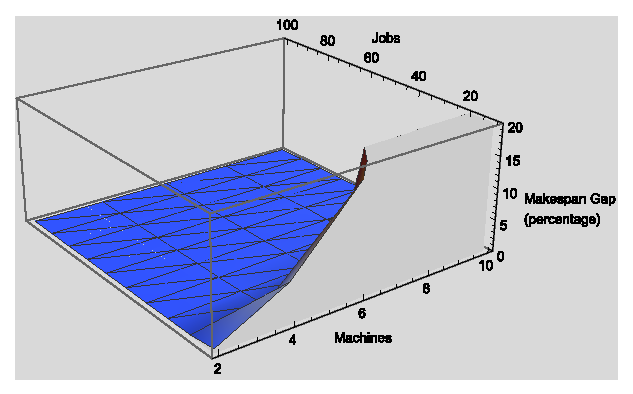
\includegraphics[width=.95\linewidth,height=.7\linewidth]{plots/Q1dRandomMakespanGap.eps}};
  \caption{Random}
  \label{fig:Q1dSFig1}
\end{subfigure}%
\begin{subfigure}{.5\textwidth}
  \centering
  \tikz[remember picture]\node[inner sep=0pt,outer sep=0pt] (rates2){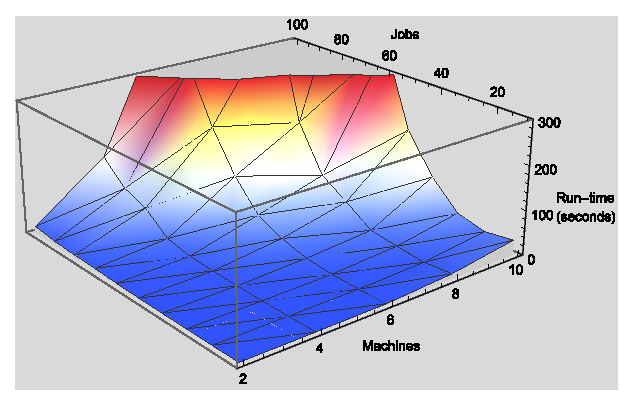
\includegraphics[width=.95\linewidth,height=.7\linewidth]{plots/Q1dRandomRunTime.eps}};
    \caption{Random}
    \label{fig:Q1dSFig2}
\end{subfigure}
\begin{subfigure}{.5\textwidth}
  \centering
 \tikz[remember picture]\node[inner sep=0pt,outer sep=0pt] (rates3){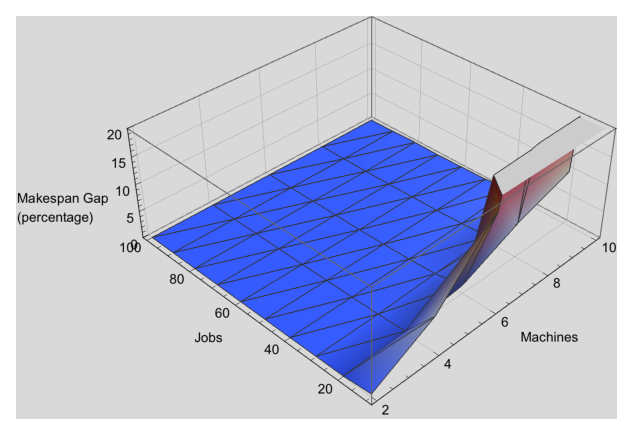
\includegraphics[width=.95\linewidth,height=.7\linewidth]{plots/Q1dGMSMakespanGap.eps}};
   \caption{GMS}
  \label{fig:Q1dSFig3}
\end{subfigure}
\begin{subfigure}{.5\textwidth}
  \centering
  \tikz[remember picture]\node[inner sep=0pt,outer sep=0pt] (rates4){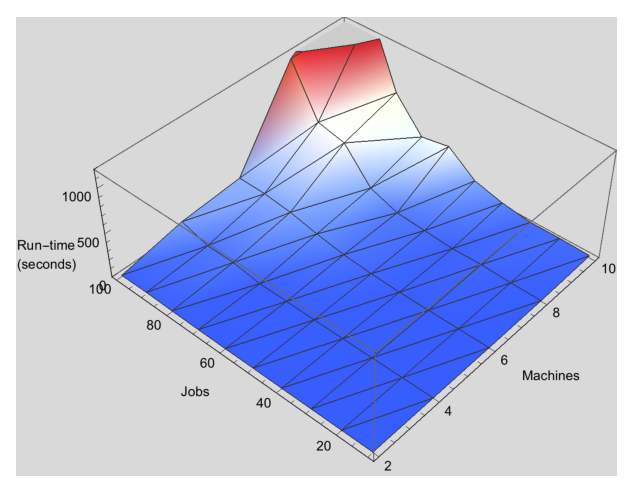
\includegraphics[width=.95\linewidth,height=.7\linewidth]{plots/Q1dGMSRunTime.eps}};
  \caption{GMS}
  \label{fig:Q1dSFig4}
\end{subfigure}
\caption[Experiments: Random and GMS]{\textbf{Experiments: k=2, using random and GMS initial solution.} \small (a) and (b) display the makespan gap (in percentage) and the run time (in seconds), using a random initial solution. (c) and (d) show makespan gap (in percentage) and the run time (in seconds), using the GMS initial solution.}
\label{fig:Q1d}

\end{figure}










\newpage













\section{Variable Depth Search Algorithm for MS}

In our Python code, we generally represent any feasible solution $\{S_1,S_2,...,S_m\}$ to the Knapsack problem as a list $\xi = [\xi_1,\xi_2,...,\xi_n]$ of length $n$, where each $\xi_i \in [1,...,m]$ which represents in which machine job $i$ is contained. Methods have been included which convert the solutions between these two representations (\textit{convertSol\_toListOfMachines} and \textit{convertSol\_toSetsOfJobs}). \\


Pseudo-code for VDS:
We begin with an input instance $I = (p_1,p_2,...,p_n,m)$ of the Knapsack problem. 
\begin{enumerate}
\item We generate an initial feasible solution $\xi = \{\xi_1,\xi_2,...,\xi_n\}$, \color{red} MENTION HOW \color{black}
\item $\textnormal{IMPROVEMENT} := \textnormal{TRUE}$
\item $\textnormal{EXCHANGE} := \{1,2,...,n\}$, $J=0$, $\alpha_J := \xi$
\item \textbf{while} $\textnormal{IMPROVEMENT} = \textnormal{TRUE}$ \textbf{do begin}
\begin{enumerate}
\item \textbf{while} $\textnormal{EXCHANGE} \neq \emptyset$ \textbf{do}
\begin{enumerate}
\item \textbf{begin} $J := J+1$
\item $\alpha_J := $ the best neighbour in the $k$-neighbourhood of $\alpha_{J-1}$. We define \textit{gain}$(\alpha_{J-1}, \delta) = \textnormal{makespan}(\alpha_{J-1}) - \textnormal{makespan}(\delta)$. Hence, the best neighbour $\alpha_J$ is defined such that \\ \textit{gain}$(\alpha_{J-1},\alpha_J) = $max$\{$\textit{gain}$(\alpha_{J-1},\delta) | \delta \in \textnormal{Neigh}_k(\alpha_{J-1}) - \{\alpha_{J-1} \}$ and $\delta$ differs from $\alpha_{J-1}$ in the parameters of $\textnormal{EXCHANGE}$ only $\}$.
\item $\textnormal{EXCHANGE} := \textnormal{EXCHANGE} - \{ \textnormal{the parameters in which } \alpha_J \textnormal{ and } \alpha_{J-1} \textnormal{ differ } \}$ (i.e., we remove the job index for which the machine has been changed from $\textnormal{EXCHANGE}$). 
\end{enumerate}
\item \textbf{end}
\item Compute \textit{gain}$(\alpha,\alpha_i) = \textnormal{makespan}(\alpha) - \textnormal{makespan}(\alpha_i)$, for $i=1,...,J$
\item Compute $l \in \{1,...,J\}$ such that \\ \textit{gain}$(\alpha,\alpha_l) = \textnormal{max}\{$\textit{gain}$(\alpha,\alpha_i) \> | i \in \{1,2,...,J\} \}$
\item \textbf{if} \textit{gain}$(\alpha,\alpha_l) > 0$ \textbf{then}
\begin{enumerate}
\item $\textnormal{EXCHANGE} := \{1,2,...,n\}$
\item \textbf{end}
\end{enumerate}
\item \textbf{else} $\textnormal{IMPROVEMENT} := \textnormal{FALSE}$
\item \textbf{end}
\end{enumerate}
\item \textbf{output}$(\alpha)$
\end{enumerate}




Say something about `differentsolrequired'








\end{document}